% Font size, paper type
\documentclass[12pt]{article}
% Aesthetic margins
\usepackage[margin=1in]{geometry}
% Core math packages,
% Mathtools loads amsmath, and amsmath gives basic math symbs
% Amsfonts & amssymb are misc. symbols you might need
\usepackage{mathtools, amsfonts, amssymb}
% Links in a pdf
\usepackage{hyperref}
% Use in pictures, graphs, and figures
\usepackage{graphicx}
% Header package
\usepackage{fancyhdr}
% Underlining with line breaks
\usepackage{ulem}
% Adjust accordingly given warning messages
\setlength{\headheight}{15pt}
% So we can more easily format text with pictures
\usepackage{float}
% Images and drawing graphs
\usepackage{tikz}

% Sets footer
\pagestyle{fancy}
% Removes default footer style
\fancyhf{}

\rhead{
  Shengdong Li
  Calc 3
}

\rfoot{
  Page \thepage{}
}

% Makes links look more appealing
\hypersetup{
    colorlinks=true,
    linkcolor=blue,
    filecolor=magenta,      
    urlcolor=cyan,
}

% \usepackage{indentfirst}

\begin{document}
\title{Macromolecule Discussion}
\author{by Shengdong Li}
\date{3 March 2021}
\maketitle

Hello everyone!

For my video I chose \href{https://www.youtube.com/watch?v=4YKFw2KZA5o}{\textit{CRISPR\: Gene editing and beyond}} from a YouTube channel named \textit{nature video}.

This video demonstrates how the shape of a protein closely determines its functionality, as well as how enzymes help catalyze metabolic processes.

\begin{figure}[H]
  \begin{center}
    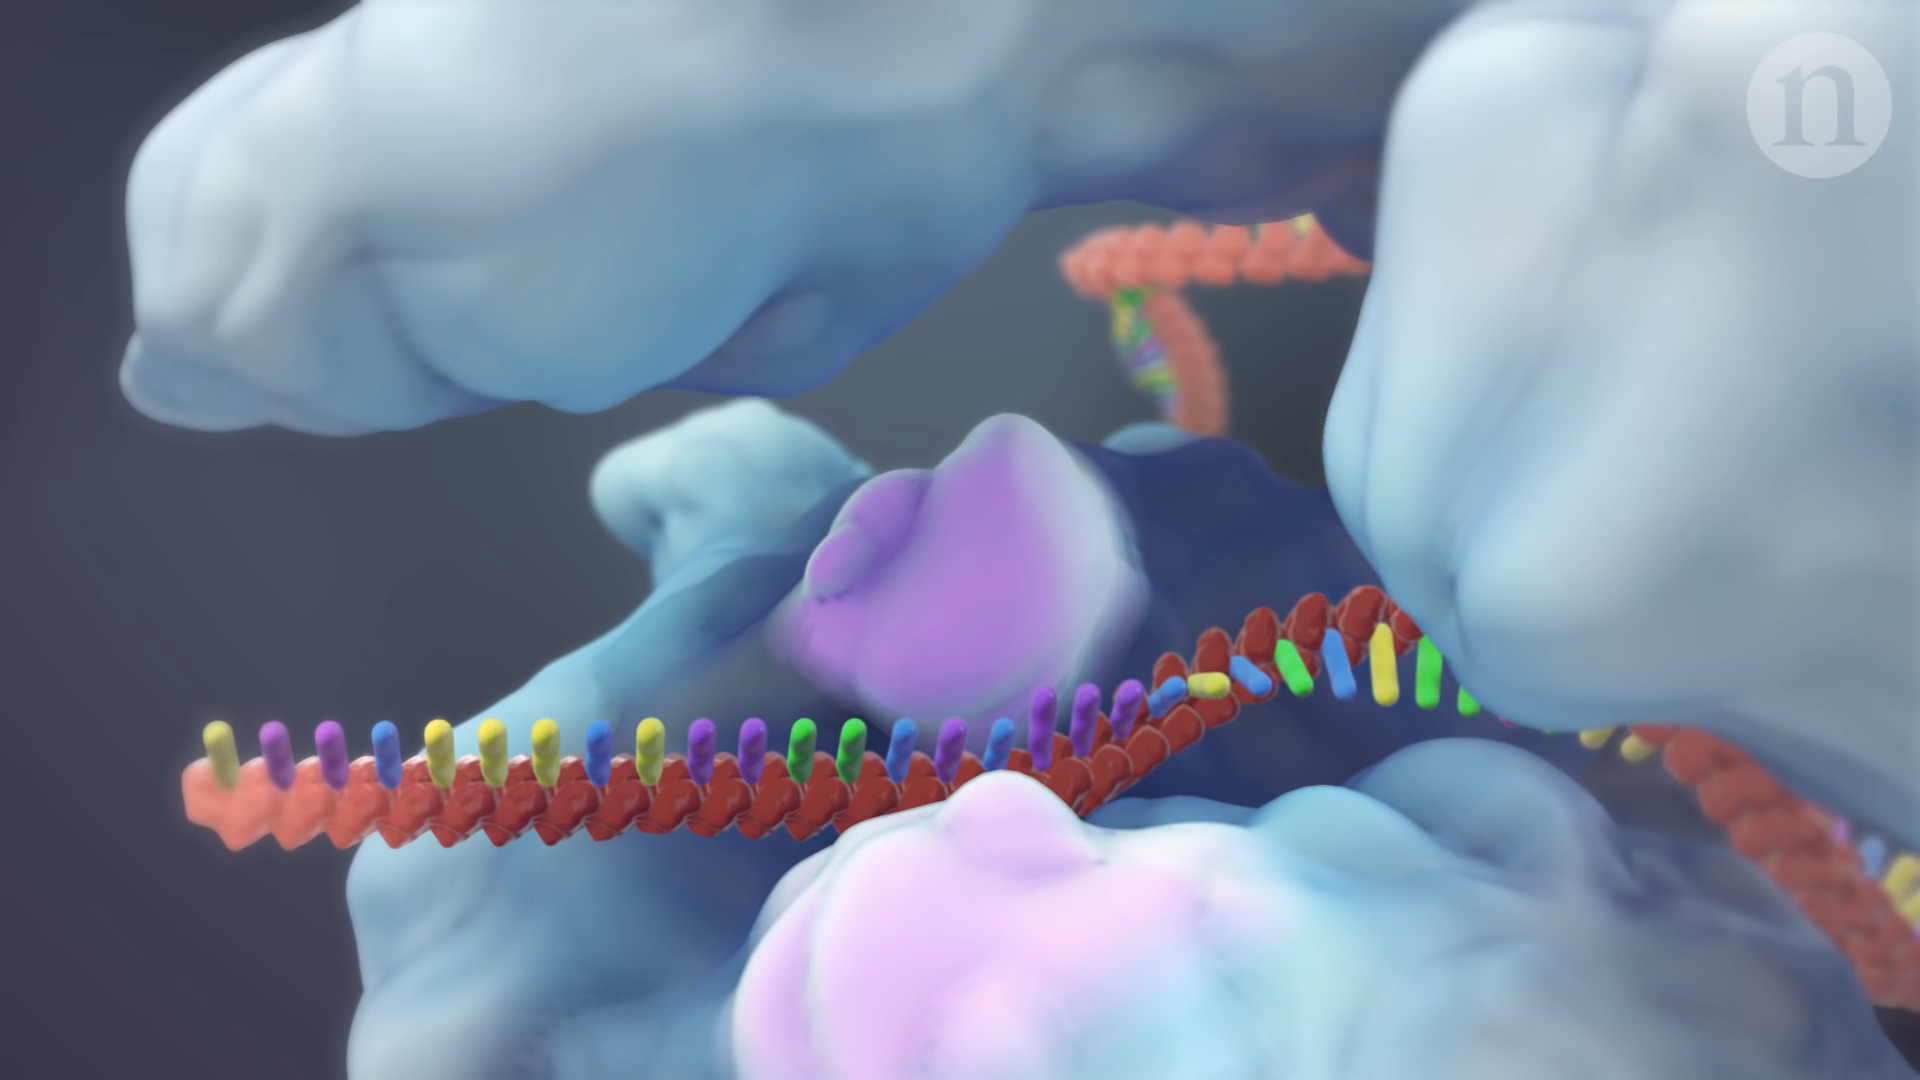
\includegraphics[scale=.2]{snapshot.jpg}
    \caption{\textit{A frame of the video demonstrating the structure of the CAS9 protein}}
  \end{center}
\end{figure}

Some background about CRISPR\: It's about DNA editing, based off a fundamental process of nature. To defend against viruses, bacteria have an immune system that save some of a viruses DNA, known as Constantly Spaced Repeating Palindromic Repeats (CRISPR). Then when new viruses arrive, the bacteria use a system known as ``CRISPR CAS9'' to defend against it. In this system, a CAS9 protein is generated uses a guide RNA (cloned from the DNA sequence of the virus that the cell saved) protein to seek out the DNA sequence in bacteria, and cut it out.

This video is about the structure of a CAS9 protein. It shows that the two cutting sites used to cut out proteins, part of the CAS9 protein's structure are integral to its cutting functionality. If the structure of the CAS9 protein is changed, the cutting sites can be made to no longer function. Then enzymes can be added to the CAS9 protein, to facilitate chemical reactions that can change the bases of the DNA sequence. The modification of the CRISPR CAS9 system and its proteins can be thus adapted for precise gene editing, it's a really fascinating video that I think is really interesting!


\end{document}